System Architect - Justin
<<<<<<< HEAD
\begin{itemize}
\item Show the architectural block diagram of translator.
Look into adding images to latex?

\item Describe the interfaces between the modules.
Dotpars interface, as seen above follows a standard form of a compiler. The raw
source file is fed into the lexer, ocamllex, which outputs a series of tokens that is then
parsed by ocamlyacc.  Ocamlyacc uses a our custom type system to output an abstract
syntax tree.

Our abstract syntax tree then undergoes a series of modifications and optimizations before it
is complied down into scala and fed into the scala compiler.  The first transform
is done by the aptly named "transform.ml" which reverses nodes with a tree.  (The lexer
recurses right to left, and thus all lists are stored backeds and need to be reversed.
The transform outputs a modified ast which is then fed into the semantic analyzer.

The semantic analyzer performs an extensive amount of type checking, making 
sense of a user's source code, throwing errors where need be, recovering from 
small errors if possible,  and adding necessary information to the symbol table.  

Next, the parallelizer, where the main optimizations are acomplished, takes 
the modified ast from the semantic analyzer and performs two passes to test. 
Each pass performs a series of tests to find, and declare certain functions as "pure".
These functions that are pure can be parallelized. Our optimizatinos focus on major
bottlenecks of source programs including maps, reduces, and list comprehensions.

Lastly, the parallelizer outputs a modified ast which is fed into the generator, 
which does a pass over the ast, translating the tree into and creating parallelized 
functions where applicable, which is lastly fed into the scala compiler.  The
scala compiler then complies down the JVM which can then be run on a target machine.

Dotpar uses a total of 5 different passes over the abstract syntax, performing 
checks and optimizations at each state to insure relability.  With this comes
the added benefit of a program not required to be parallizable to be run.  Dotpar
will only attempt to parallelize a program after extensive checks which gives add 
compile security and relability.

\item State which modules were written by which team members.
The grammar was designed and implemented Sid Nair, and Nathan Hwang, with the
conversion to Ocaml being carried out by Sid Nair and Justin Hines.  The parser was
completed by Nathan Hwang and Justin Hines.  The transform by Nathan Hwang.  The
Semantic Analyzer was implemented by Justin Hines and Andrew Hitti.  The Parallelizer was
implemented by Sid Nair with minor contributions by Justin Hines, and Nathan Hwang. 
The Geneator was implemented by Nathan Hwang with signifcant contributions from 
Sid Nair, Andrew Hitti, and Justin Hines.

\end{itemize}



=======
>>>>>>> b00e82f749b18ae63ef8250cddd1fda9c35efab0

\section{Block Diagram}
\begin{figure}[H]
\centering
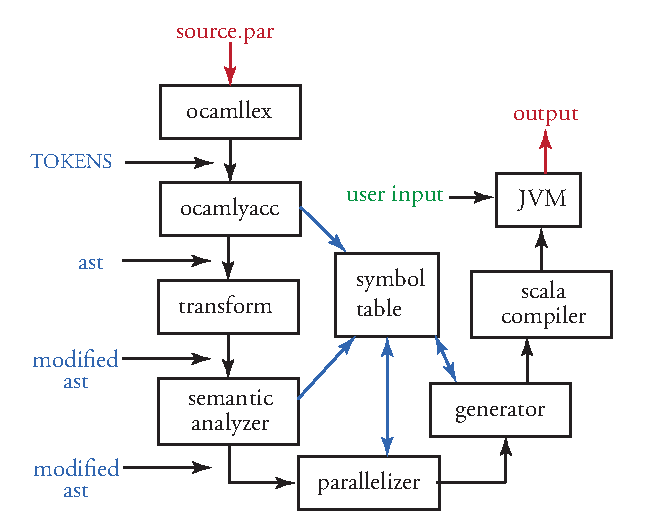
\includegraphics[scale=1]{blockdiagram.eps} 
\caption{Block Diagram of the DotPar compiler.}
\end{figure}

\section{Interfaces}
Dotpars interface, as seen above follows a standard form of a
compiler. The raw source file is fed into the lexer, \verb=ocamllex=,
which outputs a series of tokens that is then parsed by the parse,
\verb=ocamlyacc. Ocamlyacc= uses a our type system implemented in the
output a tree like ast with nested types.

Our ast is then undergoes a series of modifications and optimizations
before it is complied down into scala and fed into the scala compiler.
The first transform is done by the aptly named transform which
reverses nodes with a tree.  The lexer recurses right to left, and
thus we need to reverse this.  The transform outputs a modified ast
which is then fed into the semantic analyzer.The semantic analyzer
performs an extensive amount of type checking, making sense of the
source code, throwing errors where need be, fixing things if
necessary, and adding necessary informatino to the symbol table.
Next, the parallelizer, where the main optimizations are done, takes
our modified ast and performs two passes to test what functions, if
any can be parallelized. We focus on major bottlenecks which include
maps, reduces, and list comprehensions. Lastly, the parallelizer
outputs a modified ast which is fed into the generator, which does a
pass over the ast, translating the tree into scala which is then
lastly fed into the scala complier.

\section{Implementation}
The grammar was designed and implemented Sid Nair, and Nathan Hwang,
with the conversion to ocaml being carried out by Sid Nair and Justin
Hines.  The parser was completed by Nathan Hwang and Justin Hines.
The transform by Nathan Hwang.  The Semantic Analyzer was implemented
by Justin Hines and Andrew Hitti.  The Pallelizer was implemented by
Sid Nair, Nathan Hwang, and Justin Hines. The Generator was
implemented by Nathan Hwang with signifcant contributions from Nathan
Hwang, Andrew Hitti and Justin Hines.
